\chapter{QMDD}\label{chap:qmdd}

{\itshape Quantum Multiple-Valued Decision Diagram} é uma estrutura de dados composta de um grafo dirigido acíclico cujos vértices são rotulados para representar um dos qubits do circuito. Por meio dessas informações, é possível percorrer o grafo de forma a reconstruir completamente a matriz que ele representa. Assim, o QMDD se mostra uma forma sem perdas de compactar matrizes. Além disso, é possível manipular QMDDs e realizar operações como adição e multiplicação entre eles sem precisar reconstruir suas matrizes, fazendo com que essas operações também tirem vantagem da capacidade de compressão oferecida pelo QMDD. [QUOTE: QMDD1]

Para que o diagrama não cresça exponencialmente em relação ao número de qubits no circuito, são necessárias outras restrições cujos algoritmos devem se ater a não violar. % TODO: As regras estão a seguir:

\begin{enumerate}
  \item Existe um único vértice que não possui arestas saintes. Esse vértice é chamado de vértice terminal.
  \item Todos os vértices que não são o vértice terminal possuem um rótulo indicando qual qubit o vértice representa e um conjunto de $r^2$ arestas saintes. No caso de QMDDs para circuitos quânticos, $r=2$, logo cada vértice possui 4 arestas.
  \item Existe uma única aresta sem vértice de origem. Essa é a aresta pela qual se iniciam todas as buscas pelo grafo e aponta para o vértice chamado de inicial.
  \item Todas as arestas do grafo são ponderadas por um valor complexo.
  \item Os rótulos dos vértices são ordenáveis, de forma que os rótulos de todo caminho formado do vértice inicial ao terminal estejam ordenados. Ou seja, em uma busca pelo gráfico, sempre se encontrará os vértices de cada qubit na mesma ordem. Além disso, essa ordem diz que o qubit menos significativo do circuito é o mais próximo do vértice terminal, enquanto o mais significativo é o próprio vértice inicial.
  \item Nenhum vértice não terminal é redundante. Ou seja, nenhum vértice possui todas as suas arestas com mesmo peso e apontando para um mesmo vértice. Caso todas as arestas tenham peso 0, o vértice ainda é considerado redundante mesmo que os vértices destino sejam diferentes. Isso porque a presença de um 0 no caminho entre o vértice inicial e final anula inteiramente o valor do caminho, fazendo com que qualquer aresta com peso 0 possa levar imediatamente ao vértice terminal sem alterar o valor do QMDD.
  \item Todo nodo não terminal é sempre normalizado, de forma que a primeira aresta de valor não nulo tem sempre valor 1. Note que deve sempre existir pelo menos uma aresta não nula, pois se todas as arestas tiverem peso 0, o vértice seria redundante.
  \item Todos os vértices são únicos. Ou seja, não existe um par de vértices com mesmo rótulo e todas as arestas iguais.
\end{enumerate}

Como estabelecido na \cref{sec:matrixrep}, para que um circuito quântico possa ser convertido em matrizes para ser simulado, são necessárias 3 operações fundamentais: construção da matriz a partir da porta; multiplicação de matrizes; medição. Nesta seção, serão apresentados os algoritmos necessários para realização dessas operações, em conjunto das subrotinas necessárias para os algoritmos. Por exemplo, a multiplicação de QMDDs faz uso da subrotina de adição de QMDDs.

Além disso, também será feita uma breve introdução ao conceito de grafos, e como eles oferecem formas eficazes de percorrer dados por meio de caminhos, uma funcionalidade essencial para a manipulação e recuperação das informações contidas em QMDDs.

\section{Como Ler um QMDD}\label{sec:qmddvis}

A representação gráfica de um QMDD permite a visualização de como um determinado valor da matriz codificada pode ser extraído por meio de um caminho entre o vértice raiz e o vértice terminal. A TODO representa a matriz H. QMDDs que representam uma porta sobre um único qubit podem facilmente ser construídos, precisando apenas de um vértice inicial e um terminal, sendo as 4 arestas do vértice inicial os 4 valores presentes em cada posição da matriz. Note que ainda é necessário aplicar o algoritmo de normalização apresentado em \cref{alg:normalize} para garantir a consistência caso esse QMDD participe de uma operação com outro QMDD.

Já para matrizes que representam portas sobre múltiplos qubits, a ligação direta entre arestas e posições da matriz deixa de existir. Por exemplo, a matriz $X \otimes H$ pode ser representada com apenas 8 arestas, apesar de ser uma matriz com 16 posições, como demonstrado na TODO.

% TODO: Figura do QMDD

% TODO: Reescrever esse fuckass parágrafo
Para reconstruir a matriz representada por esse diagrama, basta seguir o caminho da aresta inicial ao vértice final. Cada vértice é rotula um qubit e suas arestas representam uma das 4 possíveis escolha para ler o qubit: começou em 0 e está em 0; começou em 1 e está em 0; começou em 0 e está em 1 ou começou em 1 e está em 1. Como os qubits normalmente são inicializados em \ket{0}, pode-se construir o caminho considerando apenas a primeira e a terceira aresta do vértice. Caso o qubit do vértice esteja em \ket{0} no estado a ser lido, segue a primeira aresta e caso esteja em \ket{1} segue a terceira.

Ao atingir o vértice terminal, basta multiplicar os pesos de todas as arestas presentes no caminho tomado para recuperar o valor representado pela matriz original.

\section{Grafos}\label{sec:graph}

Visto que QMDDs dependem integralmente de grafos, esta seção busca introduzir os conceitos necessários para compreender as definições do QMDD e as restrições necessárias para que um grafo seja válido para um QMDD. [QUOTE: livro do santiago sobre grafos]

Grafo é o nome dado para estruturas de dados organizadas em elementos e ligações entre esses elementos. Cada elemento do grafo é chamado de vértice e as ligações entre os elementos são chamadas de arestas. Um cenário no qual grafos são úteis, por exemplo, é a representação entre diferentes pontos de ônibus de uma cidade e a existência de uma rota que ligue 2 pontos. Nesse caso, cada ponto de ônibus é um vértice e sempre que exista uma linha de ônibus levando de um ponto A para um ponto B, vai existir uma aresta ligando os vértices A e B. Arestas podem ser representadas como uma tupla com o vértice de saída e o vértice destino da aresta.

O grafo da \cref{fig:graph2nodes} é composto do conjunto de vértices \{A, B\} e do conjunto de arestas \{(A, B)\}.

\begin{figure}[h]
  \centering
  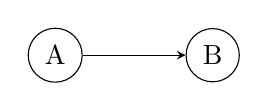
\begin{tikzpicture}[>=stealth, node distance=2cm]

  \node (A) [circle, draw] {A};
  \node (B) [circle, draw, right of=A] {B};

  \draw[->] (A) -- (B);

  \end{tikzpicture}
  \caption{Grafo com 2 vértices}
  \label{fig:graph2nodes}
\end{figure}


\subsection{Caminhos}
A existência de uma aresta saindo de A e levando a B significa que existe um caminho de A para B. Nem todos os vértices do precisam estar diretamente ligados por uma aresta, é possível que exista um caminho indireto entre dois vértices. Por exemplo, no grafo~\cref{fig:graph3node}, existe um caminho de A para B e um de B para C, isso significa que, indiretamente, também existe um caminho de A para C.

\begin{figure}[h]
  \centering
  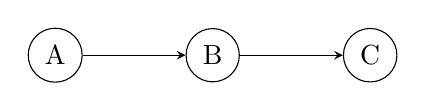
\begin{tikzpicture}[>=stealth, node distance=2cm]

  \node (A) [circle, draw] {A};
  \node (B) [circle, draw, right of=A] {B};
  \node (C) [circle, draw, right of=B] {C};

  \draw[->] (A) -- (B);
  \draw[->] (B) -- (C);

  \end{tikzpicture}
  \label{fig:graph3node}
\end{figure}

\subsection{Arestas Ponderadas}
Além de armazenar apenas a informação de que se existe ou não um caminho entre dois vértices, uma aresta também pode armazenar um valor para esse caminho. Normalmente esse valor é entendido como o custo da aresta, porém, nos QMDDs, esse valor é interpretado como um dos valores que compõem a matriz representada.

No exemplo dos pontos de ônibus, o valor de uma aresta poderia representar o tempo que leva para chegar de um lugar a outro. Isso se torna útil em junção com o conceito de caminho indireto: se o caminho de A para C é na verdade o caminho de A para B seguido do caminho de B para C, sabe-se que o custo para chegar em C a partir de A será a soma dos custos para ir de A a B e de B a C. Por exemplo, se a aresta (A, B) tem valor 10 minutos e a aresta (B, C) tem valor 20 minutos, sabe-se que é possível sair de A e chegar em C em 30 minutos.

\begin{figure}[h]
  \centering
  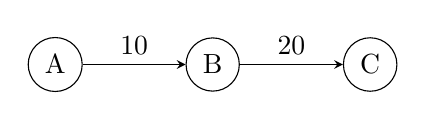
\begin{tikzpicture}[>=stealth, node distance=2cm]

  \node (A) [circle, draw] {A};
  \node (B) [circle, draw, right of=A] {B};
  \node (C) [circle, draw, right of=B] {C};

  \draw[->] (A) -- (B) node[midway, above] {10};
  \draw[->] (B) -- (C) node[midway, above] {20};

  \end{tikzpicture}
  \label{fig:graph3nodeweighted}
\end{figure}


\subsection{Grafos Dirigidos e Ciclos}
Note que a possibilidade de ir do ponto A para o ponto B não implica na existência de um caminho de B para A. Por isso a ordem da tupla é importante para as arestas. Dessa forma, grafos podem ou não ser dirigidos, ou seja, é possível impor a restrição de que toda aresta representa a existência de ambos os caminhos, tornando a ordem da tupla irrelevante. Caso o grafo não seja dirigido, toda aresta resulta na existência de um ciclo, ou seja, existe um caminho de um vértice para ele mesmo. No caso da aresta não dirigida (A, B), existe um caminho de A para B e existe um caminho de B para A, logo existe um caminho de A para A.

Por outro lado, no caso de grafos dirigidos, a existência de um ciclo passa a ser apenas uma possibilidade facilmente identificada. No caso dos QMDDs, essa restrição é sempre respeitada pela forma como os algoritmos de construção e manipulação são definidos. Porém, dado um grafo arbitrário, é possivel verificar se existe um ciclo por meio de uma busca a partir de cada vértice, verificando se existe um caminho que leve de volta ao mesmo vértice. %TODO: citar busca em profundidade

O presente grafo na \cref{fig:acyclicgraph} é acíclico, visto que não existe caminho de nenhum vértice para si mesmo, já o grafo na \cref{fig:cyclicgraph}, existe um caminho de A para A, passando pelos vértices B e C, logo esse grafo é cíclico.

\begin{figure}[h]
  \centering
  \begin{minipage}{0.45\textwidth}
    \centering
    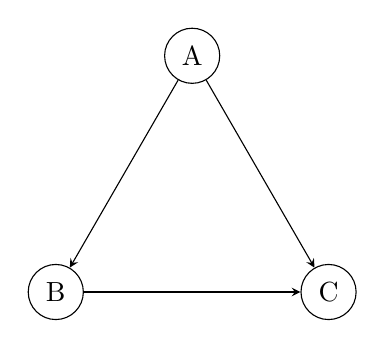
\begin{tikzpicture}[>=stealth, every node/.style={circle,draw,minimum size=7mm}]
      \node (A) at (90:2)  {A};
      \node (B) at (210:2) {B};
      \node (C) at (330:2) {C};
      \draw[->] (A) -- (B);
      \draw[->] (B) -- (C);
      \draw[->] (A) -- (C);
    \end{tikzpicture}
    \caption{Grafo acíclico}
    \label{fig:acyclicgraph}
  \end{minipage}
  \qquad
  \begin{minipage}{0.45\textwidth}
    \centering
    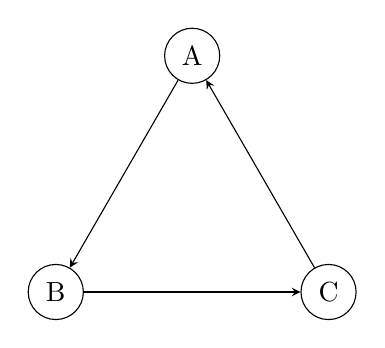
\begin{tikzpicture}[>=stealth, every node/.style={circle,draw,minimum size=7mm}]
      \node (A) at (90:2)  {A};
      \node (B) at (210:2) {B};
      \node (C) at (330:2) {C};
      \draw[->] (A) -- (B);
      \draw[->] (B) -- (C);
      \draw[->] (C) -- (A);
    \end{tikzpicture}
    \caption{Grafo cíclico}
    \label{fig:cyclicgraph}
  \end{minipage}
\end{figure}

\subsection{Representação de Vértices e Arestas}

No começo desta seção, vértices foram apresentadas como sendo elementos arbitrários de um conjunto e arestas como sendo tuplas dos vértices conectados e, opcionalmente, um peso. Para a descrição dos algoritmos do QMDD, uma notação diferente será utilizada. Nela, cada aresta possui apenas um valor e um vértice destino, enquanto cada vértice será uma tupla com seu rótulo e um conjunto de arestas.

Assim, o grafo da \cref{fig:graph3nodeweighted} pode ser representado como o conjunto de vértices $\{(A, \{(10, B)\}), (B, \{(20, C)\}), (C, \{\})\}$

\section{Algoritmos}

As operações entre QMDDs podem ser traduzidas para operações sobre suas arestas iniciais. Dessa forma, a definição recursiva para operação entre arestas é suficiente. Ao fim, essas operações retornam uma aresta que aponta para o nodo inicial do diagrama resultante da operação realizada.

\subsection{Funções Fundamentais}\label{sub:fundamentals}

Para definição sucinta dos algoritmos, serão utilizadas algumas notações para se referir a informações presentes nos vértices e arestas do QMDD.

\begin{enumerate}
  \item $x(v)$: $v$ é um vértice e $x(v)$ signfica o rótulo do vértice $v$;
  \item $v(e)$: $e$ é uma aresta e $v(e)$ representa o vértice ao qual a aresta aponta;
  \item $w(e)$: $e$ é uma aresta e $w(e)$ é o peso dessa aresta;
  \item $E_i(x)$: Quando $x$ é um vértice, $E_i(x)$ é a i-ésima aresta do vértice. Quando $x$ é uma aresta, $E_i(x)$ é a i-ésima aresta do vértice ao qual $x$ aponta;
  \item $T(e)$: $e$ é uma aresta e $T(e)$ é um valor verdadeiro ou falso que indica se a aresta é terminal. Ou seja, se o vértice ao qual $e$ aponta é o vértice terminal;
  \item $v_t$: é o vértice terminal do QMDD, que não contém nenhuma aresta.

\end{enumerate}


Além disso, note que, para representar as matrizes utilizadas por circuitos quânticos, o número de arestas por vértice do QMDD será sempre 4. Apesar de ser possível que diferentes usos de matrizes requeiram diferentes números de arestas por vértice, os algoritmos serão descritos com os valores fixos para as matrizes relevantes para a simulação de circuitos quânticos.

\subsection{Normalização e Eliminação de Redundância}

Garantir que os vértices estão normalizados é um esforço adicional para cada um dos algoritmos, visto que, por exemplo, a soma de dois vértices normalizados pode resultar em um vértice não normalizado. Imagine dois vértices, um com arestas de peso 1, 0, 0 e 1 e outro vértice com arestas de peso 0, 1, 1 e 0, todas apontadas para o mesmo vértice. Apesar de estarem normalizados, a soma dos dois vértices resultará em um vértice com arestas de peso 1, 1, 1 e 1, todas apontando para o mesmo vértice. Esse vértice por sua vez é reduntante, já que todas as arestas possuem mesmo peso e apontam para o mesmo vértice. Logo, é necessário normalizá-lo antes de retornar o resultado da soma.

\[
  \begin{tikzpicture}[
    node distance=1.5cm,
    root/.style={circle,draw,minimum size=8mm},
    leaf/.style={rectangle,draw,minimum size=6mm},
    baseline={(current bounding box.center)}
  ]

    % terminal node
    \node[leaf] (t) at (0,0) {$1$};

    % QMDD internal node
    \node[root] (v) at (0,2) {};

    % incoming edge of weight 1
    \node[above=of v] (src) {};
    \draw[->] (src) -- node[right] {$1$} (v);

    % four outgoing edges, one for each matrix entry (1,0,0,1)
    \draw[->] (v) edge[bend left=90]  node[right]  {$1$} (t); % (0,0)
    \draw[->] (v) edge[bend left=30]  node[right]  {$0$} (t); % (0,1)
    \draw[->] (v) edge[bend right=30] node[right] {$0$} (t); % (1,0)
    \draw[->] (v) edge[bend right=90] node[right] {$1$} (t); % (1,1)

  \end{tikzpicture}
  \;+\;
  \begin{tikzpicture}[
    node distance=1.5cm,
    root/.style={circle,draw,minimum size=8mm},
    leaf/.style={rectangle,draw,minimum size=6mm},
    baseline={(current bounding box.center)}
  ]

    \node[leaf] (t) at (0,0) {$1$};
    \node[root] (v) at (0,2) {};

    \node[above=of v] (src) {};
    \draw[->] (src) -- node[right] {$1$} (v);

    \draw[->] (v) edge[bend left=90]  node[right]  {$0$} (t);
    \draw[->] (v) edge[bend left=30]  node[right]  {$1$} (t);
    \draw[->] (v) edge[bend right=30] node[right] {$1$} (t);
    \draw[->] (v) edge[bend right=90] node[right] {$0$} (t);

  \end{tikzpicture}
  \;=\;
  \begin{tikzpicture}[
    node distance=1.5cm,
    root/.style={circle,draw,minimum size=8mm},
    leaf/.style={rectangle,draw,minimum size=6mm},
    baseline={(current bounding box.center)}
  ]

    \node[leaf] (t) at (0,0) {$1$};
    \node[root] (v) at (0,2) {};

    \node[above=of v] (src) {};
    \draw[->] (src) -- node[right] {$1$} (v);

    \draw[->] (v) edge[bend left=90]  node[right]  {$1$} (t); % (0,0)
    \draw[->] (v) edge[bend left=30]  node[right]  {$1$} (t); % (0,1)
    \draw[->] (v) edge[bend right=30] node[right] {$1$} (t); % (1,0)
    \draw[->] (v) edge[bend right=90] node[right] {$1$} (t); % (1,1)

  \end{tikzpicture}
  \quad\Longrightarrow\quad
  \begin{tikzpicture}[
    node distance=1.5cm,
    root/.style={circle,draw,minimum size=8mm},
    leaf/.style={rectangle,draw,minimum size=6mm},
    baseline={(current bounding box.center)}
  ]

    % terminal node
    \node[leaf] (t) at (0,0) {$1$};

    % incoming edge of weight 1
    \node[above=of t] (src) {};
    \draw[->] (src) -- node[right] {$1$} (t);

  \end{tikzpicture}
\]

A normalização de um vértice se dá por meio da aresta que aponta para esse vértice. Caso o vértice seja redundante, a aresta que aponta para ele tem seu alvo substituído para o alvo das arestas do vértice, já, caso o vértice não seja redundante, a aresta original é mantida.

Após a aplicação de cada algoritmo, é necessário normalizar novamente cada vértice de acordo com \cref{alg:normalization}. [QUOTE: QMDD1]

\begin{algorithm}[H]
  \caption{Normalização de Vértice da Aresta}
  \label{alg:normalization}
  \KwIn{Aresta $e$}
  \KwOut{Aresta}

  \If{$E_0(e) = E_1(e) = E_2(e) = E_3(e)$}{
    \Return $e_0$
  }
  \Else{
    $w \gets w(E_0(e))$ \;
    \For{$i \gets 0$ \KwTo $3$}{
      $w(E_i(e)) \gets w(E_i(e))/w$
    }
  }

  $w(e) \gets w * w(e) $

  \Return $e$

\end{algorithm}

\subsection{Multiplicação}

A multiplicação de QMDDs faz uso de uma subrotina de adição, que será apresentada antes do algoritmo em si.

\subsubsection{Adição}

A adição de dois diagramas é feita de forma recursiva, arestas que apontam para o vértice terminal têm seus valores somados, e arestas que apontam para vértices não terminais vão apontar para o resultado da soma das arestas de seus vértices alvos. [QUOTE: QMDD1]

\begin{algorithm}[H]
  \caption{Adição de Arestas}
  \label{alg:addition}
  \KwIn{Aresta $e_0$, Aresta $e_1$}
  \KwOut{Aresta}

  \If{$T(e_1)$}{
    $e_0, e_1 \gets e_1, e_0$
  }
  \If{$T(e_0)$}{
    \If{$w(e_0) = 0$}{
      \Return $e_1$
    }
    \If{$T(e_0)$}{
      $e_n \gets Aresta(w(e_0)+w(e_1), v(e_0))$ \;
      \Return $e_n$
    }
  }
  $v_n \gets Vertice(x(e_0), \emptyset)$ \;
  \For{$i \gets 0$ \KwTo $3$}{
    $p \gets Aresta(w(e_0)*w(E_i(e_0)), v(e_0))$ \;
    $q \gets Aresta(w(e_1)*w(E_i(e_1)), v(e_1))$ \;
    $E_i(v_n) \gets p + q$
  }
  \Return $normalize(Aresta(1, v_n))$

\end{algorithm}

\subsubsection{Algoritmo}

Dada a adição de duas matrizes, a multiplicação pode ser entendida como a soma das matrizes produzidas pelas convoluções das matrizes a serem somadas, logo basta multiplicar os pesos das arestas dos pares de vértices correspondentes, criando um QMDD para cada combinação de arestas e, então, somando-os. [QUOTE: QMDD2]

\begin{algorithm}[H]
  \caption{Multiplicação de Arestas}
  \label{alg:multiplication}
  \KwIn{Aresta $e_0$, Aresta $e_1$}
  \KwOut{Aresta}

  \If{$T(e_1)$}{
    $e_0, e_1 \gets e_1, e_0$
  }
  \If{$T(e_0)$}{
    \If{$w(e_0) = 0 $}{
      \Return $e_0$
    }
    \If{$w(e_0) = 1$}{
      \Return $e_1$
    }
    \Return $Aresta(w(e_0)*w(e_1), v(e_1))$
  }
  $v_n \gets Vertice(x(e_0), \emptyset)$
  \For{$i \gets 0$ \KwTo $1$}{
    \For{$j \gets 0$ \KwTo $1$}{
      $E_{2*i+j}(v_n) \gets Aresta(0, v_t)$ \;
      \For{$k \gets 0$ \KwTo $1$}{
        $p \gets Aresta(w(e_0)*w(E_{2*i+k(e_0)}), v(E_{2*i+k}(e_0)))$ \;
        $q \gets Aresta(w(e_1)*w(E_{j+2*k(e_0)}), v(E_{j+2*k}(e_1)))$ \;
        $E_{2*i+j}(v_n) \gets E_{2*i+j}(v_n) + p*q$
      }
    }
  }
  $e_n \gets normalize(Aresta(1, v_n$)) \;
  \Return $e_n$

\end{algorithm}


\subsection{Construção a Partir de Portas}\label{sec:gateconstruct}

A construção de um QMDD a partir de uma porta quântica pode ser feita de duas formas: uma porta arbitrária para um único qubit ou uma porta arbitrária controlada, com um qubit alvo e múltiplos qubits de controle.

A construção de uma porta arbitrária se dá pelo produto tensorial entre matrizes identidade e a matriz que representa a porta arbitrária, de forma a produzir uma única matriz que opere sobre todos os qubits, mantendo todos exceto o qubit alvo da porta inalterados e aplicando o efeito da porta sobre o qubit desejado. Para isso, basta utilizar o algoritmo de produto tensorial definido na \cref{subsub:kronecker}. Assim, para aplicar uma porta U no i-ésimo qubit de um circuito com k qubits, basta realizar o produto tensorial $I^{\otimes i-1} \otimes U \otimes I^{\otimes k-i}$. 

Já a construção de portas controlodas possui duas etapas: uma para os qubits de controle mais significativos que o qubit alvo e uma para os menos significativos. Essas duas etapas são descritas na \cref{subsub:controledgate} [QUOTE QMDD1, QMDD2]

\subsubsection{Produto Tensorial}\label{subsub:kronecker}

O produto tensorial consiste basicamente do encadeamento dos grafos de cada diagrama. $A \otimes B$ significa que as arestas terminais de A serão conectadas ao vértice inicial de B. Note que, por não criar novos vértices, o resultado do produto tensorial não consome mais memória que os dois valores de entrada do produto. Isso representa um ganho exponencial em relação à representação matricial do produto tensorial, cujo tamanho do resultado é o produto dos tamanhos das entradas.

\begin{algorithm}[H]
  \caption{Produto Tensorial Entre Arestas}
  \label{alg:kronecker}
  \KwIn{Aresta $e_0$, Aresta $e_1$}
  \KwOut{Aresta}
  
  \If{$T(e_0)$}{
    \If{$w(e_0) = 0$}{
      \Return $e_0$
    }
    \If{$w(e_0) = 1$}{
      \Return $e_1$
    }
    \Return $Aresta(w(e_0)*w(e_1), v(e_1))$
  }

  $v_n \gets Vertice(x(e_0), \emptyset)$ \;

  \For{$i \gets 0$ \KwTo $3$}{
    $E_i(v_n) \gets tensorial(E_i(e_0), e_1)$
  }
  \Return $normalize(Aresta(1, v_n))$
\end{algorithm}

\subsubsection{Construção de Portas Controladas}\label{subsub:controlgate}

Como dito na \cref{sec:gateconstruct}, a construção de portas controlodas se divide em duas partes: qubits de controle menos significativos que o alvo e qubits mais significativos. A construção do QMDD por meio desse método ocorre do vértice terminal ao vértice inicial, considerando apenas o qubit de controle e o qubit alvo. Para cada qubit de controle, é construído um QMDD que representa o comportamento de apenas propagar a transformação sobre o qubit alvo pelas arestas que representam o caso em que o qubit está ativo.

Note que, no caso em que não há qubits de controle, este algoritmo funciona identicamente ao algoritmo para construção de QMDDs de portas únicas, já que todos os qubits além 

\begin{algorithm}[H]
  \caption{Construção de Portas Controlodas}
  \label{alg:controlgateconstruct}
  \KwIn{Índice do qubit alvo $t$; Conjunto de índices dos qubits de controle $C$; Matriz da porta $m$}
  \KwOut{Aresta}

  $r \gets \{Aresta(v_t, m00), Aresta(v_t, m01), Aresta(v_t, m10), Aresta(v_t, m11)\}$
  $x \gets {Aresta(0, v_t), Aresta(0, v_t), Aresta(0, v_t), Aresta(0, v_t)} $

  \For{$c \in C \land c < t$}{
    \For{$i \gets \{0, 1\}$}{
      \For{$j \gets \{0, 1\}$}{
        $k \gets 2*i + j$ \;
        $x_3 \gets r_k$ \;
        $x_0 \gets Aresta(1, v_t) if i = j, else Aresta(0, v_t)$ \;
        $r_k \gets normalize(Aresta(1, Vertice(c, x)))$
      }
    }
  }
  $e \gets normalize(Aresta(1, Vertice(t, r)))$
  \For{$c \in C \land c > t$}{
    $x_3 \gets e$ \;
    $x_0 \gets Aresta(1, T)$ \;
    $e \gets normalize(Aresta(1, Vertice(c, x)))$
  }
  \Return $e$
\end{algorithm}

\subsection{Medição}\label{sub:measurement}

A operação de medição sobre o estado também pode ser representada por meio de um produto matricial. Para construir a matriz que representa essa operação, basta aplicar as matrizes $M_0$ e $M_1$, apresentadas na \cref{eq:measurementmatrices} sobre o qubit a ser medido, de acordo com o resultado obtido. Assim, pode-se tirar vantagem dos algoritmos já definidos para multiplicação de matrizes e produto tensorial para construir a matrix $I^{\otimes n-1} \otimes (M_0 ou M_1) \otimes I^{\otimes k-n}$, sendo $k$ o número de qubits no circuito e $n$ o índice do qubit medido.

\begin{equation}
  % \caption{Matrizes de Medição}
  \label{eq:measurementmatrices}
  M_0
  =
  \begin{bmatrix}
    1 & 0 \\
    0 & 0
  \end{bmatrix}
  \qquad
  M_1
  =
  \begin{bmatrix}
    0 & 0 \\
    0 & 1
  \end{bmatrix}
\end{equation}

Além disso, para extrair um resultado que obedeça à distribuição de probabilidade ao final da execução do algoritmo, é possível percorrer o grafo do vértice inicial ao final escolhendo as arestas aleatoriamente de acordo com seus pesos. Para isso, é preciso considerar apenas duas das quatro arestas dos vértices, sendo as arestas 1 e 3 responsáveis pelo resultado caso o qubit do vértice tenha sido inicializado em \ket{0} e as arestas 2 e 4 para \ket{1}. [QUOTE: QMDD2]

Esse método de obtenção de um único resultado aleatório de acordo com a distribuição probabilística do estado é chamada de simulação fraca. [QUOTE: weak simulation]

\section{Extração de Resultados}

QMMDs permitem a realização de simulação quântica forte. Isso significa que é possível extrair a probabilidade de cada resultado após a execução do circuito. Essa operação inevitavelmente possui custo exponencial, pois n qubits geram $2^n$ possíveis resultados, por isso estratégias de simulação fraca como a apresentada na \cref{sub:measurement} são utilizadas para circuitos com mais qubits. [QUOTE: strong simulation]

Caso o circuito possua uma quantia moderada de qubits, é possível realizar um procedimento semelhante à busca descrita na \cref{sub:measurement}. A diferença é que, ao invés de escolher arestas aleatoriamente, cada escolha leva ao valor que representa um resultado possível, logo basta visitar todos os caminhos possíveis.

Lembrando que o QMDD resultante do produto de todas as portas lógicas representa toda a transformação linear do circuito, envolvendo informações de resultados para circuitos inicializados em estados arbitrários e não apenas $\ket{0}^{\otimes n}$. Para extrair o resultado considerando que o circuito foi inicializado em $\ket{0}^{\otimes n}$, basta ignorar as arestas 2 e 4 de cada vértice.